%%% LaTeX-Vorlage Version 1.8 %%%

% Grundlegende Dokumenteneigenschaften gemäß DHBW-Vorgaben
\documentclass[a4paper,fontsize=11pt,oneside,parskip=half,headings=normal]{scrreprt} 
% \usepackage{showframe} % nur für Kontrolle der Ränder 

%%% Präambel einbinden (mit Festlegungen gemäß DHBW-Vorgaben) %%%
%%% Präambel %%%
% hier sollten keine Änderungen erforderlich sein
%
\usepackage[utf8]{inputenc}   % Zeichencodierung UTF-8 für Eingabe-Dateien
\usepackage[T1]{fontenc}      % Darstellung von Umlauten im PDF

\usepackage{listings}         % für Einbindung von Code-Listings
\lstset{numbers=left,numberstyle=\tiny,numbersep=5pt,texcl=true}
\lstset{literate=             % erlaubt Sonderzeichen in Code-Listings 
{Ö}{{\"O}}1
{Ä}{{\"A}}1
{Ü}{{\"U}}1
{ß}{{\ss}}2
{ü}{{\"u}}1
{ä}{{\"a}}1
{ö}{{\"o}}1
{€}{{\euro}}1
}

\usepackage[
  inner=35mm,outer=15mm,top=25mm,
  bottom=20mm,foot=12mm,includefoot
]{geometry}                 % Einstellungen für Ränder

\usepackage[ngerman]{babel} % Spracheinstellungen Deutsch
\usepackage[babel,german=quotes]{csquotes} % deutsche Anf.zeichen
\usepackage{enumerate}      % anpassbare Nummerier./Aufz.
\usepackage{graphicx}       % Einbinden von Grafiken
\usepackage[onehalfspacing]{setspace} % anderthalbzeilig

\usepackage{blindtext}      % Textgenerierung für Testzwecke
\usepackage{color}          % Verwendung von Farbe 

\usepackage{acronym}        % für ein Abkürzungsverzeichnis

\usepackage[                % Biblatex
  backend=biber,
  bibstyle=_dhbw_authoryear,maxbibnames=99,
  citestyle=authoryear,     
  uniquename=true, useprefix=true,
  bibencoding=utf8]{biblatex}
%kein Punkt am Ende bei \footcite
%http://www.golatex.de/footcite-ohne-punkt-am-schluss-t4865.html
\renewcommand{\bibfootnotewrapper}[1]{\bibsentence#1}


%Reihenfolge der Autorennamen
%   
% http://golatex.de/viewtopic,p,80448.html#80448
% Argumente: siehe http://texwelt.de/blog/modifizieren-eines-biblatex-stils/
\DeclareNameFormat{sortname}{% Bibliographie
  \ifnum\value{uniquename}=0 % Normalfall
    \ifuseprefix%
      {%
         \usebibmacro{name:family-given}
           {\namepartfamily}
           {\namepartgiveni}
           {\namepartprefix}
           {\namepartsuffixi}%
       }
      {%
         \usebibmacro{name:family-given}
           {\namepartfamily}
           {\namepartgiveni}
           {\namepartprefixi}
           {\namepartsuffixi}%
       }%
  \fi
  \ifnum\value{uniquename}=1% falls nicht eindeutig, abgek. Vorname 
      {%
         \usebibmacro{name:family-given}
           {\namepartfamily}
           {\namepartgiveni}
           {\namepartprefix}
           {\namepartsuffix}%
       }%
  \fi
  \ifnum\value{uniquename}=2% falls nicht eindeutig, ganzer Vorname 
      {%
         \usebibmacro{name:family-given}
           {\namepartfamily}
           {\namepartgiven}
           {\namepartprefix}
           {\namepartsuffix}%
       }%
  \fi   
  \usebibmacro{name:andothers}}

\DeclareNameFormat{labelname}{% für Zitate
  \ifnum\value{uniquename}=0 % Normalfall
    \ifuseprefix%
      {%
         \usebibmacro{name:family-given}
           {\namepartfamily}
           {\empty}
           {\namepartprefix}
           {\namepartsuffixi}%
       }
      {%
         \usebibmacro{name:family-given}
           {\namepartfamily}
           {\empty}
           {\namepartprefixi}
           {\namepartsuffixi}%
       }%
  \fi
  \ifnum\value{uniquename}=1% falls nicht eindeutig, abgek. Vorname 
      {%
         \usebibmacro{name:family-given}
           {\namepartfamily}
           {\namepartgiveni}
           {\namepartprefix}
           {\namepartsuffix}%
       }%
  \fi
  \ifnum\value{uniquename}=2% falls nicht eindeutig, ganzer Vorname 
      {%
         \usebibmacro{name:family-given}
           {\namepartfamily}
           {\namepartgiven}
           {\namepartprefix}
           {\namepartsuffix}%
       }%
  \fi   
  \usebibmacro{name:andothers}}
      
  
\DeclareFieldFormat{extrayear}{% = the 'a' in 'Jones 1995a'
  \iffieldnums{labelyear}
    {\mknumalph{#1}}
    {\mknumalph{#1}}}        

\renewcommand*{\multinamedelim}{\addslash}
\renewcommand*{\finalnamedelim}{\addslash}
\renewcommand*{\multilistdelim}{\addslash}
\renewcommand*{\finallistdelim}{\addslash}

\renewcommand{\nameyeardelim}{~}

% Literaturverzeichnis: Doppelpunkt zwischen Name (Jahr): Rest 
% http://de.comp.text.tex.narkive.com/Tn1HUIXB/biblatex-authoryear-und-doppelpunkt
\renewcommand{\labelnamepunct}{\addcolon\addspace}

% damit die Darstellung für Vollzitate von Primärquellen in 
% Fußnoten später auf "nicht fett" geändert werden kann 
% (nur für Zitate von Sekundärliteratur relevant)
\newcommand{\textfett}[1]{\textbf{#1}}

% für Zitate von Sekundärliteratur:
\newcommand{\footcitePrimaerSekundaer}[4]{%
  \renewcommand{\textfett}[1]{##1}%
  \footnote{\fullcite[#2]{#1}, zitiert nach \cite[#4]{#3}}%  
  \renewcommand{\textfett}[1]{\textbf{##1}}%
}

% Im Literaturverzeichnis: Autor (Jahr) fett
\renewbibmacro*{author}{%
  \ifboolexpr{%
    test \ifuseauthor%
    and
    not test {\ifnameundef{author}}
  }
    {\usebibmacro{bbx:dashcheck}
       {\bibnamedash}
       {\usebibmacro{bbx:savehash}%
        \textfett{\printnames{author}}%
        \iffieldundef{authortype}
          {\setunit{\addspace}}
          {\setunit{\addcomma\space}}}%
     \iffieldundef{authortype}
       {}
       {\usebibmacro{authorstrg}%
        \setunit{\addspace}}}%
    {\global\undef\bbx@lasthash
     \usebibmacro{labeltitle}%
     \setunit*{\addspace}}%
  \textfett{\usebibmacro{date+extrayear}}}

% Sonderfall: Quelle ohne Autor, aber mit Herausgeber
% Name des Herausgebers wird fett gedruckt
\renewbibmacro*{bbx:editor}[1]{%
  \ifboolexpr{%
    test \ifuseeditor%
    and
    not test {\ifnameundef{editor}}
  }
    {\usebibmacro{bbx:dashcheck}
       {\bibnamedash}
       {\textfett{\printnames{editor}}%
        \setunit{\addcomma\space}%
        \usebibmacro{bbx:savehash}}%
     \usebibmacro{#1}%
     \clearname{editor}%
     \setunit{\addspace}}%
    {\global\undef\bbx@lasthash
     \usebibmacro{labeltitle}%
     \setunit*{\addspace}}%
  \textfett{\usebibmacro{date+extrayear}}}

% Anpassungen für deutsche Sprache
\DefineBibliographyStrings{ngerman}{%
	nodate = {{o.J.}},
	urlseen = {{Abruf:}},
	ibidem = {{ebenda}}
}

% keine Anführungszeichen beim Titel im Literaturverzeichnis
\DeclareFieldFormat[article,book,inbook,inproceedings,manual,misc,phdthesis,thesis,online,report]{title}{#1\isdot}

\newcommand{\literaturverzeichnis}{%
% nur Literaturverzeichnis
% (als eigenes Kapitel)
\phantomsection
\addcontentsline{toc}{chapter}{Literaturverzeichnis}
\spezialkopfzeile{Literaturverzeichnis}
\defbibheading{lit}{\chapter*{Literaturverzeichnis}}
\label{chapter:quellen}
\printbibliography[heading=lit,notkeyword=ausblenden]
} % mit DHBW-spezifischen Einstellungen

\usepackage{hyperref}       % URL-Formatierung, klickbare Verweise

\usepackage{tocloft}        % für Verzeichnis der Anhänge

\usepackage{multirow}

\newcounter{anhcnt}
\setcounter{anhcnt}{0}
\newlistof{anhang}{app}{}

\newcommand{\anhang}[1]{%
  \refstepcounter{anhcnt}
  \setcounter{anhteilcnt}{0}
  \section*{Anhang \theanhcnt: #1}
  \addcontentsline{app}{section}{\protect\numberline{Anhang \theanhcnt}#1}\par
}

\newcounter{anhteilcnt}
\setcounter{anhteilcnt}{0}

\newcommand{\anhangteil}[1]{%
	\refstepcounter{anhteilcnt}
	\subsection*{Anhang~\arabic{anhcnt}/\arabic{anhteilcnt}: #1}
	\addcontentsline{app}{subsection}{\protect\numberline{Anhang \theanhcnt/\arabic{anhteilcnt}}#1}\par
}

\renewcommand{\theanhteilcnt}{Anhang \theanhcnt/\arabic{anhteilcnt}}

% vgl. S. 4 Paket-Beschreibung tocloft 	
% Einrückungen für Anhangverzeichnis
\makeatletter
\newcommand{\abstaendeanhangverzeichnis}{
\renewcommand*{\l@section}{\@dottedtocline{1}{0em}{5.5em}}
\renewcommand*{\l@subsection}{\@dottedtocline{2}{2.3em}{6.5em}}
}
\makeatother

% Abbildungs- und Tabellenverzeichnis
% Bezeichnungen
\renewcaptionname{ngerman}{\figurename}{Abb.}
\renewcaptionname{ngerman}{\tablename}{Tab.}
% Einrückungen
\makeatletter
\renewcommand*{\l@figure}{\@dottedtocline{1}{0em}{2.3em}}
\renewcommand*{\l@table}{\@dottedtocline{1}{0em}{2.3em}}
\makeatother


\usepackage{chngcntr}                % fortlaufende Zähler für Fußnoten, Abbildungen und Tabellen
\counterwithout{figure}{chapter}
\counterwithout{table}{chapter}
\counterwithout{footnote}{chapter}

\usepackage[automark]{scrlayer-scrpage} 
%% Definitionen für Kopf- und Fußzeile auf normalen Seiten
\defpagestyle{kopfzeile}
{% Kopfdefinition
  (\textwidth,0pt)    % Länge der oberen Linie,Dicke der oberen Linie       
  {} % Definition für linke Seiten im doppelseitigen Layout
  {} % Definition für rechte Seiten im doppelseitigen Layout      
  {  % Definition für Seiten im einseitigen Layout
	\makebox[0pt][l]{\rightmark}% 
	\makebox[\linewidth]{}% 
  }        
  (\textwidth, 0.4pt) % Untere Linienlänge, Untere Liniendicke
}
{% Fußdefinition
  (\textwidth,0pt)    % Obere Linienlänge, Obere Liniendicke
  {} % Definition für linke Seiten im doppelseitigen Layout
  {} % Definition für rechte Seiten im doppelseitigen Layout
  {  % Definition für Seiten im einseitigen Layout
    \makebox[\linewidth]{}%
    \makebox[0pt][r]{\pagemark}%
  }
  (\textwidth, 0pt)   % Länge der unteren Linie,Dicke der unteren Linie
}

%% Definitionen für Kopf- und Fußzeile auf ersten Seiten eines Kapitels
\defpagestyle{kapitelkopfzeile}
{% Kopfdefinition
  (\textwidth,0pt)    % Länge der oberen Linie,Dicke der oberen Linie       
  {} % Definition für linke Seiten im doppelseitigen Layout
  {} % Definition für rechte Seiten im doppelseitigen Layout      
  {}  % Definition für Seiten im einseitigen Layout
  (\textwidth, 0pt) % Untere Linienlänge, Untere Liniendicke
}
{% Fußdefinition
  (\textwidth,0pt)    % Obere Linienlänge, Obere Liniendicke
  {} % Definition für linke Seiten im doppelseitigen Layout
  {} % Definition für rechte Seiten im doppelseitigen Layout
  {  % Definition für Seiten im einseitigen Layout
    \makebox[\linewidth]{}%
    \makebox[0pt][r]{\pagemark}%
  }
  (\textwidth, 0pt)   % Länge der unteren Linie,Dicke der unteren Linie
}

%% Definitionen für Kopf- und Fußzeile im Anhang und bei Quellenverzeichnisse
\newcommand{\spezialkopfzeileBezeichnung}{}
\defpagestyle{spezialkopfzeile}
{% Kopfdefinition
  (\textwidth,0pt)    % Länge der oberen Linie,Dicke der oberen Linie       
  {} % Definition für linke Seiten im doppelseitigen Layout
  {} % Definition für rechte Seiten im doppelseitigen Layout      
  {  % Definition für Seiten im einseitigen Layout
	\makebox[0pt][l]{\spezialkopfzeileBezeichnung}% 
	\makebox[\linewidth]{}% 
  }        
  (\textwidth, 0.4pt) % Untere Linienlänge, Untere Liniendicke
}
{% Fußdefinition
  (\textwidth,0pt)    % Obere Linienlänge, Obere Liniendicke
  {} % Definition für linke Seiten im doppelseitigen Layout
  {} % Definition für rechte Seiten im doppelseitigen Layout
  {  % Definition für Seiten im einseitigen Layout
    \makebox[\linewidth]{}%
    \makebox[0pt][r]{\pagemark}%
  }
  (\textwidth, 0pt)   % Länge der unteren Linie,Dicke der unteren Linie
}
            
\newcommand\spezialkopfzeile[1]{%
  \renewcommand\spezialkopfzeileBezeichnung{#1}
  \pagestyle{spezialkopfzeile}
}
                
% Standard-Pagestyle auswählen
\pagestyle{kopfzeile}

% keine Kopfzeile anzeigen auf Seiten, auf denen ein 
% Kapitel beginnt oder das Inhalts-/Abbildungs-/Tabellenverzeichnis steht 
\renewcommand{\chapterpagestyle}{kapitelkopfzeile}
\tocloftpagestyle{kapitelkopfzeile}

		 % für schöne Kopfzeilen 

\usepackage{textcomp}            % erlaubt EUR-Zeichen in Eingabedatei
\usepackage{eurosym}             % offizielles EUR-Symbol in Ausgabe
\renewcommand{\texteuro}{\euro}  % ACHTUNG: nach hyperref aufrufen!

\usepackage{scrhack}             % stellt Kompatibilität zw. KOMA-Script
                                 % (scrreprt) und anderen Paketen her
                                 
% Anpassung der Abstände bei Kapitelüberschriften
% (betrifft auch Inhalts-, Abbildungs- und Tabellenverzeichnis)
\renewcommand*\chapterheadstartvskip{\vspace*{-\topskip}}
\newcommand{\myBeforeTitleSkip}{1mm}
\newcommand{\myAfterTitleSkip}{10mm}
\setlength\cftbeforetoctitleskip{\myBeforeTitleSkip}
\setlength\cftbeforeloftitleskip{\myBeforeTitleSkip}
\setlength\cftbeforelottitleskip{\myBeforeTitleSkip}

\setlength\cftaftertoctitleskip{\myAfterTitleSkip}
\setlength\cftafterloftitleskip{\myAfterTitleSkip}
\setlength\cftafterlottitleskip{\myAfterTitleSkip}                                                            
%%% Ende der Präambel %%%


%%% Name der eigenen Literatur-Datenbank (ggf. anpassen) %%%
\bibliography{includes/pa1.bib}

\begin{document}
%%% Deckblatt einbinden %%% 
% Anpassungen nötig (Name, Titel etc.)
% HIER EDITIEREN: 
% Typ der Arbeit (für Deckblatt und ehrenwörtliche Erklärung)
% - bitte Zutreffendes auswählen
\newcommand{\typMeinerArbeit}{1. Projektarbeit} 
%\newcommand{\typMeinerArbeit}{2. Projektarbeit} 
%\newcommand{\typMeinerArbeit}{Seminararbeit} 
% \newcommand{\typMeinerArbeit}{Bachelorarbeit} 

% Thema der Arbeit (für ehrenwörtliche Erklärung, ohne Umbrüche)
% HIER EDITIEREN: 
\newcommand{\themaMeinerArbeit}{Was ist ein Chatbot?}

% Vorname, Name der Autorin/des Autors (für Titelseite und Metadaten)
% HIER EDITIEREN:
\newcommand{\meinName}{Max Weiberle}

\thispagestyle{empty}

\begin{spacing}{1}
\begin{center}	
~\vspace{0mm}

% HIER EDITIEREN: Titel der Arbeit
{\sffamily
\LARGE  
% \Large  % bei sehr langen Titeln ggf. etwas kleinere Schriftart wählen
\textbf{Was ist ein Chatbot?}

\bigskip
\textbf{}
}


\vspace{15mm}

% Typ wird automatisch eingefügt (oben festlegen)
{\Large \typMeinerArbeit}

\vspace{1cm}

% HIER ggf. EDITIEREN
vorgelegt am 18. Mai 2022

\vspace{15mm}

Fakultät Wirtschaft
\medskip

Studiengang Wirtschaftsinformatik
\medskip

% HIER EDITIEREN: Kurs eintragen
Kurs WWI2021G

\vspace{10mm}

von

\vspace{10mm}

% Vorname und Name wird automatisch eingefügt (oben festlegen) 
{\large\textsc{\meinName}}

\vspace{10mm}
\end{center}

\vfill

% HIER EDITIEREN: Name des Unternehmens, Name der Betreuerin/des Betreuers
\begin{tabular}{ll}
Betreuer in der Ausbildungsstätte: & DHBW Stuttgart: \\
\hspace{0.4\linewidth} & \\
Komm.ONE & Prof., Dr., Manfred Sander \\
Stefan Fuchs \\
Studierendenbetreuer \\
\\
Unterschrift der Betreuerin/des Betreuers \\
\end{tabular}


\vspace{1cm}
%(etwas Platz für die Unterschrift der Betreuerin/des Betreuers aus der Ausbildungsstätte)
\end{spacing}

% falls ein Vertraulichkeitsvermerk erforderlich ist,
% die Kommentarzeichen in den nachfolgenden Zeilen entfernen:
 
%\begin{center}
%\small
%\textbf{Vertraulichkeitsvermerk}:
%Der Inhalt dieser Arbeit darf weder als Ganzes noch in Auszügen \\
%Personen außerhalb des Prüfungs- und Evaluationsverfahrens zugänglich gemacht werden, sofern keine anders lautende Genehmigung des Dualen Partners vorliegt. 
%\end{center}

% Meta-Daten für PDF-Datei basierend auf obigen Angaben
\hypersetup{pdftitle={\themaMeinerArbeit}}
\hypersetup{pdfauthor={\meinName}}
\hypersetup{pdfsubject={\typMeinerArbeit\ DHBW Stuttgart \the\year}}


%%% Umstellung der Seiten-Nummerierung auf i, ii, iii ... %%%
\pagenumbering{Roman}

\cleardoublepage

%%% Inhalts-, Abbildungs-, Tabellenverzeichnisse %%%
% sollen einzeilig gesetzt werden, um Platz zu sparen 
\begin{spacing}{1}
	\tableofcontents
	\clearpage
	\chapter*{Abkürzungsverzeichnis}
\addcontentsline{toc}{chapter}{Abkürzungsverzeichnis}

Ein Abkürzungsverzeichnis ist optional. Das Paket \verb|acronym| kann weit mehr, als hier gezeigt.\footnote{siehe \url{http://ctan.org/pkg/acronym}}
Beachten Sie allerdings, dass Sie die Einträge selbst in sortierter Reihenfolge angeben müssen.

\begin{acronym}[DHBW] 
% Argument definiert die Breite der ersten Spalte anhand des längsten vorkommenden Eintrags
\acro{CRM}{Customer Relationship Management}
\acro{DHBW}{Duale Hochschule Baden-Württemberg}
\acro{IEEE}{Institute of Electrical and Electronics Engineers}
\acro{ITIL}{IT Infrastructure Library}
\acro{RoI}{Return-On-Invest}
\acro{UCS}{Universal Character Set}
\acro{UTF-8}{8-Bit UCS Transformation Format} 
\end{acronym}

\vspace{2em}
{\footnotesize
\textbf{Ergänzende Bemerkung:}
Eine im Text verwendete Abkürzung sollte bei ihrer ersten Verwendung erklärt werden. Falls Sie sich nicht selbst darum kümmern möchten, kann das das Paket \verb|acronym| übernehmen und auch automatisch Links zum Abkürzungsverzeichnis hinzufügen. Dazu ist an allen Stellen, an denen die Abkürzung vorkommt, \verb|\ac{ITIL}| zu schreiben. 

Das Ergebnis sieht wie folgt aus: 
\begin{itemize}
\item erstmalige Verwendung von \verb|\ac{ITIL}| ergibt: \ac{ITIL},
\item weitere Verwendung von \verb|\ac{ITIL}| ergibt: \ac{ITIL}
\end{itemize}
Wo benötigt, kann man mit dem Befehl \verb|\acl{ITIL}| wieder die Langfassung ausgeben lassen: \acl{ITIL}.

Falls man die Abkürzungen durchgängig so handhabt, kann man durch Paket-Optionen (in \verb|_dhbw_praeambel.tex|)
erreichen, dass im Abkürzungsverzeichnis nur die tatsächlich verwendeten Quellen aufgeführt werden (Option: \verb|printonlyused|) und zu jedem Eintrag die Seite der ersten Verwendung angegeben wird (Option: \verb|withpage|).
}

	\clearpage
	\thispagestyle{kapitelkopfzeile}
	\listoffigures
	\phantomsection
	\addcontentsline{toc}{chapter}{Abbildungsverzeichnis} % Abb.verz. ins Inh.verz. aufnehmen

	\clearpage
	\listoftables
	\phantomsection
	\addcontentsline{toc}{chapter}{Tabellenverzeichnis}   % Tab.verz. ins Inh.verz. aufnehmen

  \clearpage
  \chapter*{Gender Disclaimer} % (fold)
\label{cha:Gender Disclaimer}
\addcontentsline{toc}{chapter}{Gender Disclaimer}

Aus Gründen der besseren Lesbarkeit wird auf die gleichzeitige Verwendung der Sprachformen männlich, weiblich und divers (m/w/d) verzichtet. Sämtliche Personenbezeichnungen gelten gleichermaßen für alle Geschlechter.

% chapter (end)

\end{spacing}

%%% Umstellung der Seiten-Nummerierung auf 1, 2, 3 ... %%%
\cleardoublepage
\pagenumbering{arabic}

%%% Ihr eigentlicher Inhalt %%%
% Empfehlung: strukturieren Sie Ihren Text in einzelnen Dateien 
% und binden Sie diese hier mit \input{includes/dateiname.tex} ein

\chapter{Einleitung} % (fold)
\label{cha:Einleitung}

Durch die Corona-Pandemie und die damit verbundene Entwicklung möglichst viel im Homeoffice zu arbeiten wurde die Verwendung von VPN-Verbindungen für uns bereits zum Alltag. Zudem kommt die sich ankündigende Energiekrise. Da ein Anstieg der Energiekosten um 50 Prozent aktuell als realistisch betrachtet wird und von 30.000 Menschen gesprochen wird, die noch dieses Jahr arbeitslos werden könnten, scheint es wichtiger denn je zu sein Energiekosten zu sparen. \footcite[Vgl.][]{Gries.2022} Energieexperten berufen sich auf Studien, die eine Einsparung von bis zu fünf Prozent durch Homeoffice vorhersagen. \footcite[Vgl.][S. 1 f.]{Thaler.2022} Des Weiteren haben sich Homeoffice und flexible Arbeitszeiten zu starken Kriterien für die Berufswahl entwickelt. Besonders junge Menschen legen großen Wert darauf. Millenials würden Umfragen zu Folge doppelt so häufig den Arbeitsplatz wechseln als Babyboomer, wenn sie mit der zeitlichen oder örtlichen Flexibilität nicht zufrieden sind. \footcite[Vgl.][S. 1 f.]{Hahn.2021}

Für die Firma Komm.One, als regionales Dienstleistungsunternehmen, die das Rechenzentrum von Baden-Württemberg betreut und für einen möglichst reibungslosen Ablauf in den Rathäusern und Kommunen des Landes sorgt, ist es essentiell eine zuverlässige und beständige Arbeit zu leisten. Das ist nur möglich, wenn die Belegschaft durchgängig arbeiten kann. In den letzten zwei Jahren und vor allem zu den Corona-Hochzeiten konnte dies an den Standorten nicht gewährleistet werden, da bei der Infektion einer Person alle Kontaktperson in Quarantäne mussten. Als IT Firma blieb also die Möglichkeit des Homeoffice als sinnvolle Alternative. In dieser Zeit hat sich gezeigt, dass Homeoffice sowohl Vor- als auch Nachteile gegenüber dem zuvor standardmäßigen Arbeiten vor Ort hat. Je nach Aufgabe und Verantwortung ist dies natürlich unterschiedlich. Für die Komm.One hat sich das Homeoffice als wertvolle und auch in Zukunft interessante Alternative bestätigt. Aktuell haben allein am Standort Reutlingen etwa 180 von 250 Mitarbeitern einen Homeoffice-Vertrag, der bis zu fünf Homeoffice-Tage ermöglicht.

Um diese Menge an Homeoffice möglich zu machen, ist bei der Komm.One eine VPN-Infrastruktur gewachsen, die aus historischen Gründen, auf die in der Arbeit genauer eingegangen wird, nicht optimal ist und überarbeitet werden muss. Es werden nur für interne Mitarbeiter aktuell drei verschiedene VPN-Lösungen verwendet. Deshalb verfolgt die Komm.One das Ziel einer Harmonisierung der internen VPN-Struktur durchzuführen. In dieser Arbeit sollen die möglichen VPN-Lösungen evaluiert und die für die Komm.One beste Lösung gefunden werden.

% chapter (end)

\chapter{Firewalls und VPN} % (fold)
\label{cha:Firewalls und VPN}

Um die Rolle, die VPN in nahezu allen Unternehmen spielt verstehen zu können, müssen erst ein paar grundlegende Informationen zu Netzwerken erläutert und verstanden werden.

\section{Firewalls} % (fold)
\label{sec:Firewalls}

Grundsätzlich ist eine Firewall alles, Hardware, Software oder eine Kombination aus beidem, was die Übertragung von digitalen Paketen filtern kann. Dem liegen zwei Sicherheitsfunktionen zu Grunde:

\begin{description}
	\item Filtern von Paketen: Digitale Pakete, die durch die Firewall in das zu schützende Netzwerk hinein, aber auch aus dem zu schützenden Netzwerk hinaus wollen werden auf Basis der erstellten Sicherheitsregeln gefiltert.
	\item Anwendungsproxy: Schützt individuelle Computer und ermöglicht dennoch das Nutzen von Netzwerkdiensten. Hierfür wird der IP-Informationsfluss unterbrochen. \footcite[Vgl.][S. 99]{WHITMAN.2018}
\end{description}

\begin{figure}[htb]
	\centering
	
\includegraphics[width=9cm]{graphics/dhbw.png}
	\caption[Idee eines Firewall-Systems]{Idee eines Firewall-Systems. \footnotemark}
	\label{abb:Firewall}
\end{figure}
\footnotetext{Entnommen aus: \cite[S. 357]{Pohlmann.2022}}

In Abbildung \ref{abb:Firewall} ist die erste Funktion gut zu erkennen. Die Firewall lässt die grüne Verbindung durch, weil sie nach den Sicherheitsrichtlinien in Ordnung ist, während die orangene Linie abgeblockt wird. Ein schöner Vergleich ist hier der Pförtner oder Sicherheitspersonal am Eingang. Sie kümmern sich darum, dass die bestehenden Regeln eingehalten werden. Alle Personen müssen durch dafür vorgesehene Bereiche das Gebäude betreten oder verlassen, werden auf ihre Zugangsberechtigung geprüft und müssen durch einen Metalldetektor gehen und potenziell gefährliche Dinge abgeben. Falls es zu einem Sicherheitsfehler kommt und eine Person die Kontrolle umgeht muss eine Warnung ausgegeben werden und ein anderes Team sich um das Problem kümmern. Analog dazu funktioniert auch die Firewall, welche kontrolliert über welche Protokolle und Dienste zugegriffen wird und wer mit wem kommunizieren darf. All diese Daten werden protokolliert. \footnotemark
\footnotetext{Vgl. \cite[S. 100]{WHITMAN.2018} und \cite[S. 358]{Pohlmann.2022}}

Folgende Aufgaben haben Firewall-Systeme im Allgemeinen:

\begin{itemize}
	\item Einschränken von Zugriffen von außerhalb des Netzwerks: Die offensichtlichste Gefahr ist der Angriff von außerhalb auf das eigene Netzwerk. Aus diesem Grund muss eine Firewall jedes einzelne Paket auf die individuell festgelegten Regeln überprüfen.
	\item Einschränken von unautorisierten Zugriffen von innerhalb des Netzwerks: In manchen Fällen ist es einfacher ein Netzwerk vor äußeren Einflüssen zu schützen als vor den Gefahren, die von unaufmerksamen Arbeitnehmern ausgehen können. Besonders zu beachten sind hier beispielsweise mobile Datenträger, die infizierte Dateien in das System einschleusen können. Besonders häufig kommen auch E-Mail Angriffe mit infizierten, oder ausführbaren Dateien, die beim Herunterladen oder Ausführen das gesamte Netzwerk betreffen können.
	\item Zugangskontrolle auf Nutzerebene: Es wird überprüft, welche Nutzer über das Firewall-System mit welchen Systemen kommunizieren dürfen.
	\item Zugangskontrolle auf Datenebene: Es wird überprüft, welche Daten eines definierten Nutzers und Systems über das Firewall-System übertragen werden dürfen.
	\item Rechteverwaltung: Es wird festgelegt, mit welchen Protokollen und Diensten und zu welchen Zeiten über das Firewall-System kommuniziert werden darf.
	\item Kontrolle auf Anwendungsebene: Es wird überprüft, ob Aktivitäten stattfinden, die nicht zu Anwendungen oder definierten Aufgabenstellungen gehören, generell unerwünscht sind oder Schaden am System verursachen können. Beispiele hierfür wären Spam oder Malware.
	\item Entkopplung von Diensten: Dienste werden vom Netzwerk entkoppelt, um zu verhindern, dass Fehler oder Sicherheitslücken der einzelnen Dienste zu erfolgreichen Angriffen führen können.
	\item Beweissicherung und Protokollauswertung: Jegliche Verbindungen und sicherheitsrelevante Ereignisse werden protokolliert. Diese können für die Erkennung von Sicherheitsverletzungen und zur Beweissicherung von Handlungen der Nutzer ausgewertet werden.
	\item Alarmierung: Besondere sicherheitsrelevante Ereignisse werden dem Security-Management gemeldet, so dass im Ernstfall schnell gehandelt werden kann.
	\item Verbergen der internen Netzstruktur: Im Idealfall ist aus dem unsicheren Netz heraus nicht zu erkennen, wie das zu schützende Netz strukturiert ist oder wie viele Systeme sich in diesem Netz befinden. \footnotemark
\end{itemize}
\footnotetext{Vgl. \cite{WHITMAN.2018} S. 103 ff. und \cite{Pohlmann.2022} S. 359 f.}

Allerdings ist es bei Weitem nicht mit einer Firewall getan. Um die Sicherheit eines Netzwerkes so hoch wie möglich zu halten, müssen mehrere Sicherheitssysteme zusammenarbeiten.

% section Firewalls (end)

\section{VPN} % (fold)
\label{sec:VPN}

Ein weiterer Schritt um das zu schützende Netz sicherer zu machen, aber vor allem auch um ganz neue Möglichkeit zu eröffnen ist das Einrichten von VPN-Verbindungen. Diese Technologie ermöglicht nicht nur einen Zusammenschluss von zwei Netzwerken, die an verschiedenen geografischen Standorten existieren. Zunehmend gewinnt auch die Verwendung im Bereich von Homeoffice immer mehr an Relevanz. VPN ermöglicht es mehrere Netzwerke, wie in Abbildung \ref{abb:VPN-Modell} dargestellt, oder Geräte zu einem Netzwerk zusammenzufassen, ohne dass sie nebeneinander sein müssen oder durch ein Kabel verbunden werden. In den allermeisten Fällen wird das Internet als Verbindung zwischen den Netzwerken oder Geräten verwendet. Hier wird die Verbindung über ein unsicheres Netz mit einem Tunnel dargestellt. Um diese Verbindungen brauchbar und sicher zu machen, ist eine Verschlüsselung essentiell. \footcite[Vgl.][S. 261 ff.]{WHITMAN.2018}

\begin{figure}[htb]
	\centering
	
\includegraphics[width=12cm]{graphics/dhbw.png}
	\caption[Vereinfachtes Modell eines VPN-Aufbaus]{Vereinfachtes Modell eines VPN-Aufbaus \footnotemark}
	\label{abb:VPN-Modell}
\end{figure}
\footnotetext{Entnommen aus: \cite{WHITMAN.2018} S. 296}

Die Verschlüsselung kann bildlich wie ein Tunnel verstanden werden und eine VPN-Verbindung wird häufig auch als VPN-Tunnel bezeichnet. Die beiden Router mit IPSec zeigen genau diese Verschlüsselung. IPSec ist eine in der IT weit verbreitete Verschlüsselungsmethode und der aktuelle Standard. \footnotemark
\footnotetext{Vgl. \cite{o.V..2020} und \cite{Pohlmann.2022} S. 403 ff. auch im Folgenden}

\begin{figure}[htb]
	\centering
	
\includegraphics[width=10cm]{graphics/dhbw.png}
	\caption[Realisierungsformen von IPSec]{Realisierungsformen von IPSec \footnotemark}
	\label{abb:IPSec}
\end{figure}
\footnotetext{Entnommen aus: \cite{Pohlmann.2022} S. 411}

Für einen Verbindungsaufbau werden, wie in Abbildung \ref{abb:IPSec} dargestellt, entweder zwei IPSec-Clients, zwei IPSec-Gateways oder jeweils ein Gateway und ein Client benötigt.

% section VPN (end)

% chapter (end)

\chapter{Relevanz} % (fold)
\label{cha:Relevanz}

\section{Vorteile gegenüber herkömmlichen Systemen} % (fold)
\label{sec:Vorteile gegenüber herkömmlichen Systemen}

In der nachfolgenden Abbildung (Abb \ref{abb:VorteileChatbotsPolen})

\begin{figure}[htb]
  \centering
  
\includegraphics[width=12cm]{graphics/dhbw.png}
  \caption[Vorteile für Firmen bei Verwendung von Chatbots im Kundenservice für Unternehmen in Polen]{Vorteile für Firmen bei Verwendung von Chatbots im Kundenservice für Unternehmen in Polen. \footnotemark}
  \label{abb:VorteileChatbotsPolen}
\end{figure}
\footnotetext{Entnommen aus: \cite{Bisser.2021}}

Werden die Vorteile der Verwendung von Chatbots aufgezeigt und deren Wirksamkeit. \\
Als die zwei größten Vorteile zeigt die Abbildung die eingesparte Zeit beim Kontaktieren von Kunden und die Möglichkeit Kunden rund um die Uhr betreuen zu können.

% section Vorteile gegenüber herkömmlichen Systemen (end)

\section{Nachteile gegenüber herkömmlichen Systemen} % (fold)
\label{sec:Nachteile gegenüber herkömmlichen Systemen}

In der nachfolgenden Abbildung (Abb \ref{abb:NachteileChatbots})

\begin{figure}[htb]
  \centering
  
\includegraphics[width=12cm]{graphics/dhbw.png}
  \caption[Nachteile bei der Verwendung eines Chatbots aus Sicht der Kunden]{Nachteile bei der Verwendung eines Chatbots aus Sicht der Kunden. \footnotemark}
  \label{abb:NachteileChatbots}
\end{figure}
\footnotetext{Entnommen aus: \cite{.2021}}

Werden, die laut Kunden, größten Nachteile von Chatbots aufgelistet und nach Häufigkeit sortiert.

% section Nachteile gegenüber herkömmlichen Systemen (end)

% chapter (end)

\chapter{Entscheidungsfindung} % (fold)
\label{cha:Entscheidungsfindung}

\section{Verwendete Methoden} % (fold)
\label{sec:Verwendete Methoden}

Verwendete Methoden
Um eine fundierte und stichhaltige Entscheidung treffen zu können und diese auch angemessen begründen zu können, haben wir uns für eine Nutzwertanalyse entschieden.

Eine Nutzwertanalyse ist eine Methode zur Entscheidungsfindung und wird häufig in komplexen Situationen verwendet, wenn beispielsweise viele verschiedene Aspekte und Meinungen betrachtet werden müssen. \footcite[Vgl.][S. 1 auch im Folgenden]{Kuhnapfel.2019} Sie beruht auf dem Prinzip der „Fragmentierung“, das bedeutet das Gesamtproblem wird in einzelne Teilprobleme aufgeteilt, die, wenn dies sinnvoll ist, noch einmal in ihre Teilprobleme aufgeteilt werden können. Dieses intuitive Modell wird häufig unterbewusst angewendet, wenn wir beispielsweise entscheiden wohin wir in den Urlaub möchten. Es können objektive Informationen, wie in diesem Beispiel Kosten oder Freizeitangebote, aber auch subjektive, wie Vorlieben für Essen oder Unterkunft betrachtet und miteinander abgewogen werden. \footcite[Vgl.][S. 43]{Dittmer.1995}

Durch das Erstellen einer Nutzwertanalyse wird dieser unterbewusste Prozess in den Vordergrund gebracht und der Fokus auf die Transparenz der Ergebnisse gelegt. Des Weiteren bewirkt die Fragmentierung eine Entemotionalisierung des Problems. Die Teilprobleme lenken von der emotionalen Bindung oder von einer spontanen Präferenz der Gesamtlösung ab und können leichter rational betrachtet und diskutiert werden. Dies ist vor allem der Fall, wenn der Anteil der Teillösung an der Gesamtlösung nicht klar ist. \footcite[Vgl.][S. 2]{Kuhnapfel.2019} Besonders der tendenziellen Präferenz sich für die Konstanz und gegen Veränderung zu entscheiden, wird hier entgegengewirkt.
Für eine zielführende Durchführung einer Nutzwertanalyse ist eine klar festgelegte Struktur notwendig, an der sich orientiert werden kann. Der erste und wichtigste Schritt ist die Ableitung des Zielsystems. \footcite[Vgl.][S. 44 f. auch im Folgenden]{Dittmer.1995} Ein Zielsystem setzt sich aus den bestimmten Kriterien zusammen und sollte eindeutige und objektive Beschreibungen der Wirkungen und Konsequenzen von Alternativen erlauben und alle relevanten Wertevorstellungen der Entscheidungsträger umfassen. Bei der Findung helfen Prozessfragen, wie beispielsweise „Welche Wirkungen werden beabsichtigt?“, „Worauf wirken die Alternativen?“, oder „Welche Wirkungen sollen vermieden werden?“.

Im Anschluss werden Ausschluss- und Auswahlkriterien definiert. Hier beginnt man mit Ausschlusskriterien, diese werden nicht in die Nutzwertanalyse mit einfließen, sondern schließen die Alternative kategorisch aus (auch K.O. Kriterien genannt). Auswahlkriterien können grundsätzlich in Leistungs-, Kosten-, und Terminkriterien eingeteilt werden, wobei in dieser Arbeit noch fachspezifische Kriterien betrachtet werden. \footnotemark
\footnotetext{Vgl. \cite{Wikipedia.2022} und \cite{FfEMunchen.2022}}
Eine Menge von 10-20 Kriterien wird als sinnvoll betrachtet, vor allem um zu verhindern, dass später besprochene Kriterien oberflächlicher behandelt und diskutiert werden als zu Beginn besprochene. \footcite[Vgl.][S. 8]{Kuhnapfel.2019}

Folgende Anforderungen werden an Kriterien in einer Nutzwertanalyse gestellt: \footnotemark
\footnotetext{Vgl. \cite{Kuhnapfel.2019} und \cite{Wikipedia.2022} auch im Folgenden}

\begin{description}
	\item \emph{Vollständigkeit:} Die Kriterien müssen das Problem vollständig umfassen, es darf also kein relevanter Aspekt für das Problem ausgelassen werden.
	\item \emph{Bewertbarkeit:} Kriterien sollten insofern bewertbar sein, als dass sie entweder qualitativ oder quantitativ erfassbar oder messbar sind, oder alle Teilnehmenden über das nötige Hintergrundwissen verfügen müssen, um eine informierte Bewertung abgeben zu können. Alternativ kann mit Enthaltungen gearbeitet werden, wenn beispielsweise ein sehr technischer und ein wirtschaftlicher Teil von zwei verschiedenen Abteilungen beurteilt wird.
	\item \emph{Relevanz:} Die Kriterien sollten für das in Frage stehende Problem relevant sein. Hier kann allerdings häufig keine eindeutige Aussage getroffen werden, da Teilnehmende hier eventuell andere Ansichten haben und oft keine objektive Antwort vorliegt.
	\item \emph{Reproduzierbarkeit:} Die verwendeten Kriterien sollten in ihrer Bewertung reproduzierbar sein. Das ist beispielsweise nicht der Fall, wenn die Verlässlichkeit einer Bank betrachtet wird und diese aktuell durch einen Sturm so verwüstet wurde, dass sie vorerst nicht handlungsfähig ist. Solange der Grund für die Unbeständigkeit nicht am Zielsystem selbst liegt ist das Kriterium unbrauchbar.
\end{description}

Im nächsten Schritt wird jedem Kriterium eine Gewichtung zu geordnet. Auch hier finden verschiedene Methoden Anwendung. Die einfachste aber auch ungenaueste Methode ist das „Ranking“, oder „Direct Ranking“. Hierbei wird jedem Kriterium ein Rang gegeben. Der Bereich der Aufstellung spielt hier keine große Rolle, ist im Beispiel (Abb. \ref{abb:DirectRanking}) aber mit 0-10 definiert.

\begin{figure}[htb]
	\centering
	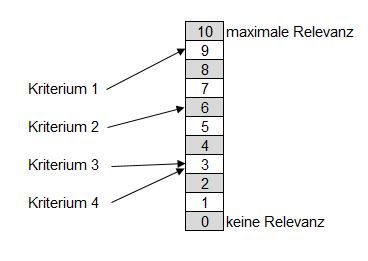
\includegraphics[width=5cm]{graphics/Direct_Ranking_Methode.JPG}
	\caption[Grafisches Beispiel Direct Ranking]{Grafisches Beispiel Direct Ranking. \footnotemark}
	\label{abb:DirectRanking}
\end{figure}
\footnotetext{Entnommen aus \cite{Wikipedia.2022}}

Die Kriterien 1-4 werden zwischen 0 (keine Relevanz) und 10 (maximale Relevanz) einsortiert. Diese Methode wird häufig verwendet, da sie so einfach ist und schnell erstellt werden kann, allerdings nimmt die Aussagekraft mit steigender Kriterienzahl stark ab. Zudem wird jedes Kriterium isoliert für sich betrachtet. Das bedeutet, es ist nicht möglich zu überprüfen inwiefern die Gewichtung passend ist. \footnotemark
\footnotetext{Vgl. \cite{PhilippsUniversitatMarburg.2013} und \cite{Wikipedia.2022}}

Des Weiteren kann durch ein sogenanntes Rating eine Gewichtung bestimmt werden. Bei diesem Verfahren kann man entweder eine Gesamtpunktzahl („Point Allocation“) auf die Kriterien aufteilen, beispielsweise 100 Punkte auf fünf Kriterien mit der Gewichtung 35, 30, 20, 10, 5. Die andere Möglichkeit ist die Verhältnisschätzung („Ratio Estimation“). Jedes Kriterium kann hier einer beliebigen Zahl aus dem Wertebereich zugeordnet werden. Das unwichtigste Kriterium beispielsweise der Punktzahl null, das wichtigste die zehn. \footcite[Vgl. ][]{PhilippsUniversitatMarburg.2013}

Für Nutzwertanalysen mit vielen Kriterien (ab ca. 20 definitiv) ist die Paarvergleichsmethode sehr sinnvoll.

\begin{table}[htb]
	\centering
	\begin{tabular}{|l||l|l|l|l|l|l|l||l|}
		\hline
		\textbf{Kriterium} & A & B & C & D & E  & F & G & $\sum$      \\
		\hline \hline
		A                  & ~ & 7 & 4 & 2 & 5  & 9 & 4 & \textbf{31} \\
		\hline
		B                  & 3 & ~ & 3 & 7 & 10 & 6 & 5 & \textbf{34} \\
		\hline
		C                  & 6 & 7 & ~ & 8 & 8  & 9 & 6 & \textbf{44} \\
		\hline
		D                  & 8 & 3 & 2 & ~ & 7  & 5 & 3 & \textbf{28} \\
		\hline
		E                  & 5 & 0 & 2 & 3 & ~  & 3 & 4 & \textbf{17} \\
		\hline
		F                  & 1 & 4 & 1 & 5 & 7  & ~ & 8 & \textbf{26} \\
		\hline
		G                  & 6 & 5 & 4 & 7 & 6  & 2 & ~ & \textbf{30} \\
		\hline
	\end{tabular}
	\caption[Kreuztabelle zur Gewichtung von Kriterien mit \glqq Ist-wichtiger-als \glqq -Stimmen]{Kreuztabelle zur Gewichtung von Kriterien mit \glqq Ist-wichtiger-als \grqq -Stimmen. \footnotemark}
	\label{tab:KreuztabelleKriterien}
\end{table}
\footnotetext{Entnommen aus \cite{Kuhnapfel.2019} S. 15}

Hier wird, wie in Tabelle \ref{tab:KreuztabelleKriterien} beispielhaft dargestellt, eine Kreuztabelle erstellt. Alle Teilnehmenden sollten einzeln bestimmen, welches Kriterium sie jeweils für wichtiger halten. Die Ergebnisse werden dann vom Moderator zusammengestellt und präsentiert. In diesem Fall haben zehn Teilnehmer abgestimmt. Logischerweise werden Kriterien nicht mit sich selbst verglichen, deshalb sind diese Felder ausgegraut. Die Ergebnisse sind hier in der letzten Spalte dargestellt und sind die Summe der „Ist-wichtiger-als“-Stimmen pro Kriterium. Im letzten Schritt wird wie in Tabelle \ref{tab:ErgebnisKreuztabelle} das Beispiel weitergeführt. Mit Hilfe eines Dreisatzes werden die Ergebnisse in ein Verhältnis gebracht und die Gewichtung berechnet. \footcite[Vgl. ][S. 13 ff.]{Kuhnapfel.2019}

\begin{table}
	\centering
	\begin{tabular}{l|l|l}
		~              & Stimmen & Gewicht(\%) \\
		\hline \hline
		Kriterium A    & 31      & 14,7        \\
		\hline
		Kriterium B    & 34      & 16,2        \\
		\hline
		Kriterium C    & 44      & 21,0        \\
		\hline
		Kriterium D    & 28      & 13,3        \\
		\hline
		Kriterium E    & 17      & 8,1         \\
		\hline
		Kriterium F    & 26      & 12,4        \\
		\hline
		Kriterium G    & 30      & 14,3        \\
		\hline
		\textbf(Summe) & 210     & 100         \\
		\hline
	\end{tabular}
	\caption[Ergebnis der Kriteriengewichtung auf Basis der Kreuztabelle]{Ergebnis der Kriteriengewichtung auf Basis der Kreuztabelle \footnotemark}
	\label{tab:ErgebnisKreuztabelle}
\end{table}
\footnotetext{Entnommen aus \cite{Kuhnapfel.2019} S. 16}

Bevor nun die Kriterien bewertet werden können, muss eine Skala bestimmt werden. Grundsätzlich hat die Skala keine Auswirkungen auf das Ergebnis der Nutzwertanalyse. Dennoch ist davon abzuraten sehr kleine oder sehr große Skalen zu definieren. Kleine Skalen bieten zu wenig Differenzierbarkeit, große hingegen können dafür sorgen, dass Teilnehmende, die zu Polarisierung neigen, mehr Einfluss auf das Ergebnis nehmen, als diejenigen, die sich tendenziell an der „goldenen Mitte“ orientieren. Die sicherlich einfachsten und verständlichsten Skalen sind die 0-10 Skala und die Schulnotenskala. Beide eignen sich hervorragend für eine Nutzwertanalyse. \footnotemark
\footnotetext{Vgl. \cite{Kuhnapfel.2019} S. 16 ff., \cite{Dittmer.1995} S. 49 f. und \cite{FfEMunchen.2022}}

Um eine Nutzwertanalyse verwendbar und aussagekräftig zu machen sollte sie reproduzierbar sein. Dies kann nur durch eine ausführliche und gewissenhaft geführte Dokumentation gewährleistet werden. Diese soll für Außenstehende ein nachvollziehbarer Nachweis sein. Zum einen soll eine Nutzwertanalyse mit anderen Teilnehmenden, an anderen Standorten oder zu einem anderen Zeitpunkt wiederholt werden können. \footnotemark
\footnotetext{Vgl. \cite{Kuhnapfel.2019} S. 4 f. und \cite{Wikipedia.2022}}

In der Dokumentation sollen harte und weiche Faktoren so erklärt werden, dass beide nachvollziehbar sind. Harte Faktoren können mit betriebswirtschaftlichen Kennzahlen belegt werden. Man spricht hier von ökonomischer Objektivierung durch Kennziffern. Weiche Faktoren hingegen beinhalten beispielsweise Erfahrungswerte, Images, Stimmungen und Handlungsweisen. Sie sind nicht oder nur mit Hilfsindikatoren als Kennzahlen darstellbar und ergeben sich aus der Diskussion. \footcite[Vgl. ][S. 1 f.]{Prof.Dr.JanLies.2018}

% section Verwendete Methoden (end)

\section{Durchführung} % (fold)
\label{sec:Durchführung}

Da im Haus schon mehrere VPN-Lösungen im Gebrauch sind, die auch für eine Harmonisierung in Frage kommen, war recht schnell klar, was die Auswahlmöglichkeiten für das Entscheidungsproblem sind. Für die Harmonisierung der VPN-Einzelplätze für interne Mitarbeiter der Komm.One kommen die Checkpoint-VPN Lösung und die NCP-VPN Lösung in Frage. Anyconnect-VPN, was auch in der Firma verwendet wird wurde bereits im Voraus aussortiert und wird im Folgenden nicht mehr betrachtet. Der enorme Aufwand eines kompletten Neuaufbaus und die damit verbundenen Kosten konnten den anderen beiden Alternativen von vornerein keine Konkurrenz machen.

Um alle benötigten Kriterien zu finden, haben wir die Methode des „Brainstorming“ verwendet. Daraus entstand folgende Liste: Fixe Kosten, Laufende Kosten, Anschaffungskosten Software, Anschaffungskosten Hardware, Softwarekosten einmalig, Softwarekosten laufend, Betriebskosten, Implementierungskosten, Migrationskosten, Kosten Kunde einmalig, Kosten Kunde laufend – Supportkosten, Skalierungskosten, Mitarbeiterkosten, Shared Service Kosten, Kostensumme innerhalb der nächsten 5 Jahre, Fortbildungskosten, Zeitaufwand Umstellung, Zeitaufwand Support, Einrichtung, Supportaufwände im Kalenderjahr, Supportaufwände einzeln, Administrationsaufwände, Rest-API (Funktion), Interkonnektivität (Funktion), Nutzung für Kunden, Self-Service Möglichkeiten, Sicherheit, Zuverlässigkeit, Handhabung, Anwenderfreundlichkeit und Verwaltungsfreundlichkeit.

Mit dieser Liste konnten wir dann weiterarbeiten. Sinn eines „Brainstormings“ ist es natürlich nicht sich viele Gedanken über die einzelnen Punkte zu machen, sondern möglichst alles, was den Beteiligten einfällt, fest zu halten. Viele dieser Punkte bedingen sich gegenseitig, oder meinen schlichtweg Dasselbe. Diese müssen natürlich entfernt werden. Einige der Punkte haben sich im Verlauf des Verfahrens als irrelevant, oder nicht umfangreich genug herausgestellt. Bei einigen wurde uns auch bewusst, dass sie genauer definiert werden müssen, um Missverständnisse zu vermeiden.

Ergebnis des Überarbeitungsprozesses ist die Tabelle \ref{tab:FinalKriterien}.

\begin{table}
	\centering
	\begin{tabular}{l|l|}
		                                       & \textbf{Kriterien}                  \\
		\hline \hline
		\multirow{10}{6em}{\textbf{Kosten}}    & Anschaffungskosten Software         \\
		~                                      & Anschaffungskosten Hardware         \\
		~                                      & Fortbildungskosten                  \\
		~                                      & Laufende Softwarekosten             \\
		~                                      & Laufende Hardwarekosten             \\
		~                                      & Mitarbeiterkosten einmalig          \\
		~                                      & Mitarbeiterkosten laufend           \\
		~                                      & Supportkosten                       \\
		~                                      & Skalierungskosten                   \\
		~                                      & Kosten für Fremdleistungen          \\
		\cline{2-2}
		\multirow{6}{6em}{\textbf{Aufwand}}    & Zeitaufwand Vorbereitung            \\
		~                                      & Zeitaufwand Implementierung         \\
		~                                      & Zeitaufwand Support                 \\
		~                                      & Anzahl Supportfälle im Kalenderjahr \\
		~                                      & Zeitaufwand pro Supportfall         \\
		~                                      & Administrationsaufwände             \\
		\cline{2-2}
		\multirow{2}{6em}{\textbf{Funktionen}} & Rest-API/Schnittstelle              \\
		~                                      & Interkonnektivität                  \\
		\cline{2-2}
		\multirow{7}{6em}{\textbf{Andere}}     & Self-Service                        \\
		~                                      & Sicherheit                          \\
		~                                      & Zuverlässigkeit                     \\
		~                                      & Anwenderfreundlichkeit              \\
		~                                      & Verwaltungsfreundlichkeit           \\
		~                                      & Fehlertoleranz Admin                \\
		~                                      & Fehlertoleranz Benutzer             \\
		\cline{2-2}
	\end{tabular}
	\caption[Finale Aufstellung aller verwendeten Kriterien für die Nutzwertanalyse]{Finale Aufstellung aller verwendeten Kriterien für die Nutzwertanalyse}
	\label{tab:Kriterien}
\end{table}

Die Punkte Anschaffungskosten Software und Hardware sind selbsterklärend, ebenso wie laufende Software- und Hardwarekosten. Bei den Fortbildungskosten geht es um Kosten für Schulungen für die Mitarbeiter, die bisher mit einer der anderen Lösungen gearbeitet haben. Mitarbeiterkosten einmalig bezieht sich auf die Kosten, die durch die Umstellung einmalig entstehen, während Mitarbeiter laufend die benötigten Mitarbeiter für den dauerhaften Betrieb der jeweiligen Lösung bewerten soll. Unter dem Kriterium Supportkosten wird bewertet, wie gut die jeweilige Alternative in Bezug auf die Menge an Supportanfrage an den Hersteller und die damit verbundenen Zusatzkosten ist. Auf den ersten Blick scheinen Kosten für Fremdleistungen hier das gleiche zu meinen, allerdings betrachten wir unter diesem Aspekt nicht die Kosten für Supportfälle und andere Unregelmäßigkeiten, sondern die Kosten, die regelmäßig für Arbeiten am System entstehen, aber nicht intern durchgeführt werden können. Skalierungskosten bezieht die Möglichkeit in Betracht das System in Zukunft erweitern zu können. Wie teuer wäre es beispielsweise das System um 500 Clients zu erweitern?

Zeitaufwände für Vorbereitung beschreibt den benötigten Zeitaufwand vor der Harmonisierung, um diese überhaupt möglich zu machen. Beim Zeitaufwand für Implementierung ist vor allem der Aspekt der Fehlerbehebung wichtig. Wie groß wird der Aufwand sein, um bei allen Mitarbeitern eine erneut funktionierende VPN-Verbindung aufbauen zu können? Zeitaufwand Support beschreibt die benötigte Zeit, die Mitarbeitende mit Supportfällen anderer Mitarbeitenden aufwenden müssen. Hierunter fallen auch Kleinigkeiten, wie Passwort vergessen oder ähnliches. Anzahl Supportfälle im Kalenderjahr und Zeitaufwand pro Supportfall sind aufgelistet der Vollständigkeit und Transparenz wegen, finden aber, wie später noch einmal genauer erläutert, keine eigene Gewichtung, sondern fließen unter dem Punkt Zeitaufwand Support in die Wertung mit ein. Drei Kriterien, die den gleichen Aspekt bewerten, verzerren das Ergebnis, wenn sie vollständig in das Ergebnis einfließen. Der Aspekt Support wäre deutlich wichtiger gewertet als gewünscht. Beispielsweise können zwei Alternativen hier eine ähnliche Bewertung was den Zeitaufwand für Support angeht bekommen, aber aus komplett verschiedenen Gründen. Bei Alternative A gibt es im Jahr nur zwei bis drei Supportfälle, diese sind aber immer sehr aufwendig und beanspruchen teilweise sogar mehrere Tage. Alternative B hat hingegen viele Supportfälle, die sich allerdings immer innerhalb einer halben Stunde beheben lassen. Da beide Alternativen in Summe auf ähnliche Zeitaufwände für Support kommen, ist die Bewertung zwar gleich, die Gründe hierfür sind allerdings so verschieden, dass wir das auch noch in Betracht ziehen wollen. Administrationsaufwände bezieht sich auf die Möglichkeiten Administrationsarbeiten, wie Updates oder sicherheitsrelevante Arbeiten durchzuführen.

Bei Rest-API/Schnittstelle geht es um eine Programmierschnittstelle, die das Verbinden mit Cloud-Diensten und Interaktionen ermöglicht. Bei dem Aspekt Interkonnektivität betrachten wir welche Geräte bzw. Betriebssysteme unterstützt werden. Speziell, ob Android- und Apple-Geräte unterstützt werden.

Self-Service bewertet die Möglichkeit, dass Mitarbeitende kleine Supportfälle, wie beispielsweise ein vergessenes Passwort und damit verbundenes gesperrtes Konto, selbst beheben können. Natürlich ist einer der wichtigsten Aspekte die Sicherheit. Anwenderfreundlichkeit bezieht sich zu großen Teilen auf persönliche Präferenzen, ebenso wie die Verwaltungsfreundlichkeit. Die Aspekte Fehlertoleranz Admin und Benutzer sollen bewerten, wie schlimm ein Fehler der jeweiligen Gruppe oder Person wäre und wie groß die Auswirkungen eines Fehlers potenziell sind.

Im nächsten Schritt wird die Gewichtung der Entscheidungskriterien betrachtet und bewertet. Hier bedienen wir uns keiner der bereits genannten Methoden direkt. Als Vorbild dient das Entscheidungsformular der Firma Komm.One, in der eine kleine und relativ oberflächliche Tabelle vorgegeben ist. Die Tabelle unterscheidet die Kriterien Kunden-/Anwenderperspektive, Finanzperspektive, Prozessperspektive, Personal-/Potenzialperspektive, Markenwirkung/Image, Recht/Compliance und Konsequenzen/Synergien/Effekte. Die Tabelle gibt Prioritäten von 0 (spielt keine Rolle), 1 (kaum Einfluss), 2 (beachtenswert) und 3 (starker Einfluss) vor. Pro Kriterium kann dann die beste Alternative gekennzeichnet werden und es wird ein Ergebnis berechnet. Eben diese Gewichtung von null bis drei haben wir uns zu Nutze gemacht, dabei handelt es sich um eine Verhältnisschätzung.

Das Ergebnis zeigt Tabelle \ref{tab:Gewichtungen}. Wir haben uns gegen eine Gewichtung der einzelnen Kriterienkategorien entschieden (daher alle auf eins gesetzt), da ansonsten die Ergebnisse noch stärker auseinandergehen und dies nicht mehr repräsentativ für den Vergleich der Lösungen wäre. Anschaffungskosten haben wir jeweils mit zwei bewertet, da Kosten, vor allem so große, immer wichtig sind, es sich aber um einmalige Kosten handelt und es unser Ziel war, die auf lange Sicht, beste Lösung zu finden. Fortbildungskosten werden in unserer Nutzwertanalyse zwar noch geführt, aber durch die Gewichtung von null fließt die Bewertung nicht in das Gesamtergebnis ein. Entfernen wollten wir es, ähnlich wie bei der Anzahl Supportfälle und Zeitaufwand pro Supportfall nicht, um eine möglichst hohe Transparenz zu erreichen. Die Nutzwertanalyse soll zeigen, dass diese Aspekte berücksichtigt wurden, jedoch in unserem Fall keinen Einfluss auf das Ergebnis haben sollen. Bei den laufenden Kosten haben wir uns auch jeweils für eine Gewichtung von zwei entschieden, obwohl es sich um immer wiederkehrende Kosten handelt, weil wir hier ein bisschen mit den Grenzen der Gewichtungsskala in Berührung kommen. Wir sind der Meinung, dass die laufenden Kosten wichtiger sind als die Anschaffungskosten, vor allem auf lange Sicht. Allerdings sind sie nicht so wichtig wie eindeutige dreier Gewichtungen wie laufende Mitarbeiterkosten oder die Sicherheit. Da in unserer Skala keine Wertung zwischen zwei und drei möglich ist haben wir uns dafür entschieden auch die laufenden Kosten mit zwei zu gewichten. In unseren Augen ist die Differenz zu einer dreier Gewichtung höher als zu einer zweier. Einmalige Mitarbeiterkosten sehen wir als nicht so wichtig an und haben deshalb eine eins vergeben. Die bereits erwähnten laufenden Mitarbeiterkosten, Supportkosten und Kosten für Fremdleistungen müssen eindeutig mit drei gewichtet werden. Grund dafür ist, dass es sich hierbei um die größten Kostenpunkte handelt. Der Aspekt der Skalierungskosten wird mit zwei gewichtet, weil auch hier die Relevanz auf lange Sicht auf jeden Fall gegeben ist, aber eine Gewichtung mit drei nicht gerechtfertigt ist.

\begin{table}
	\centering
	\begin{tabular}{l|l|l|}
		                                       & \textbf{Kriterien}                  & \textbf{Gewichtung} \\
		\hline \hline
		\multirow{10}{6em}{\textbf{Kosten}}    & Anschaffungskosten Software         & 2                   \\
		~                                      & Anschaffungskosten Hardware         & 2                   \\
		~                                      & Fortbildungskosten                  & 2                   \\
		~                                      & Laufende Softwarekosten             & 2                   \\
		~                                      & Laufende Hardwarekosten             & 2                   \\
		~                                      & Mitarbeiterkosten einmalig          & 2                   \\
		~                                      & Mitarbeiterkosten laufend           & 2                   \\
		~                                      & Supportkosten                       & 2                   \\
		~                                      & Skalierungskosten                   & 2                   \\
		~                                      & Kosten für Fremdleistungen          & 2                   \\
		\cline{2-3}
		\multirow{6}{6em}{\textbf{Aufwand}}    & Zeitaufwand Vorbereitung            & 2                   \\
		~                                      & Zeitaufwand Implementierung         & 2                   \\
		~                                      & Zeitaufwand Support                 & 3                   \\
		~                                      & Anzahl Supportfälle im Kalenderjahr & 0                   \\
		~                                      & Zeitaufwand pro Supportfall         & 0                   \\
		~                                      & Administrationsaufwände             & 2                   \\
		\cline{2-3}
		\multirow{2}{6em}{\textbf{Funktionen}} & Rest-API/Schnittstelle              & 1                   \\
		~                                      & Interkonnektivität                  & 2                   \\
		\cline{2-3}
		\multirow{7}{6em}{\textbf{Andere}}     & Self-Service                        & 2                   \\
		~                                      & Sicherheit                          & 3                   \\
		~                                      & Zuverlässigkeit                     & 3                   \\
		~                                      & Anwenderfreundlichkeit              & 3                   \\
		~                                      & Verwaltungsfreundlichkeit           & 3                   \\
		~                                      & Fehlertoleranz Admin                & 0                   \\
		~                                      & Fehlertoleranz Benutzer             & 3                   \\
		\cline{2-3}
	\end{tabular}
	\caption[Gewichtung der Kriterien mit der Skala 0-3]{Gewichtung der Kriterien mit der Skala 0-3}
	\label{tab:Gewichtungen}
\end{table}

Was den Zeitaufwand für die Vorbereitung und für die Implementierung angeht, haben wir uns auch hier für eine Gewichtung von zwei entschieden. Die Kriterien müssen natürlich in einem Verhältnis zum Nutzen der Umstellung stehen, sollen allerdings nicht entscheidend für das Endergebnis sein. Sicherlich einer der wichtigsten Punkte und ein großer Grund wieso die Harmonisierung vorangetrieben wird, sind die Supportaufwände für die jeweilige Alternative. Deshalb wird dieses Kriterium zweifelsohne mit drei gewichtet. Allerdings setzt sich hier das Kriterium aus den zwei nachfolgend aufgeführten Kriterien zusammen, die wir, wie bereits erwähnt, der Vollständigkeit und Transparenz wegen mit in der Nutzwertanalyse führen, sie aber nicht im Einzelnen in das Ergebnis einfließen lassen. Den Aspekt der Administrationsaufwände haben wir mit zwei gewichtet, mit einer ähnlichen Begründung, wie bei den laufenden Kosten. Es handelt sich definitiv um einen wichtigen Punkt, allerdings in unseren Augen nicht wichtig genug für eine Gewichtung von drei.
Die Funktion Rest-API/Schnittstelle haben wir mit eins bewertet, da sie einem einiges an Arbeit abnehmen und das Arbeiten vereinfachen kann, aber nicht notwendig ist. Die Interkonnektivität zwischen Geräten bzw. Betriebssystemen wird mit zwei gewichtet. Innerhalb der Firma wird größtenteils mit Windows gearbeitet, da aber einzelne Mac oder Linux Geräte vorhanden sind ist es sicherlich ein Aspekt der beachtet werden muss.

Self-Service Möglichkeiten orientieren sich zwar stark an dem Gedankengang, der bei der Rest-API/Schnittstelle Anwendung gefunden hat. Allerdings haben wir uns hier für eine Gewichtung von zwei entschieden, da dies abgesehen von den „Nice-To-Have“-Gründen enormen Einfluss auf Supportaufwände und -kosten haben kann. Sicherheit muss ohne Frage eine drei zugeordnet werden, ebenso wie der Zuverlässigkeit. Mit Zuverlässigkeit ist hier nicht nur die dauerhafte Möglichkeit einen VPN-Tunnel aufbauen zu können oder die Beständigkeit des Tunnels nach dem Aufbau gemeint, sondern auch die Redundanz bei Fehlern im System. Es darf beispielsweise nicht sein, dass der Ausfall eines Standortes für einen Zusammenbruch des ganzen Netzwerks führt und kein Mitarbeiter mehr arbeiten kann. Zusammen mit der Anwenderfreundlichkeit und der Verwaltungsfreundlichkeit können auch diese Aspekte alle Einfluss auf die Supportaufwände und –kosten haben und werden deshalb mit drei gewichtet. Fehlertoleranz des Admins ist ein weiterer Punkt, den wir der Vollständigkeit und Transparenz wegen aufgenommen haben, der aber nicht in das Ergebnis miteinfließt. Der Grund ist hier ganz klar, dass ein Admin mit jedem System, dass er betreut so umgehen kann, dass angemessen damit gearbeitet wird. Anders sieht das bei der Fehlertoleranz der Benutzer aus. Diesen Aspekt sehen wir auch aufgrund der Auswirkungen auf die Aspekte Supportaufwände und –kosten, aber auch direkt auf die Mitarbeiterkosten laufend als sehr wichtig und haben ihn deshalb mit drei gewichtet.

% section Durchführung (end)

\section{Ergebnisse} % (fold)
\label{sec:Ergebnisse}

% TODO: Verweise einfügen
Folgende Bewertungen haben wir vergeben (Tab. 5 und Tab. 6).

\begin{table}
	\centering
	\begin{tabular}{l|l|l|l|r|}
		\textbf{Checkpoint}                    & \textbf{Kriterien}                  & \textbf{Gewichtung} & \textbf{Bewertung} & \textbf{Ergebnis} \\
		\hline \hline
		\multirow{10}{6em}{\textbf{Kosten}}    & Anschaffungskosten Software         & 2                   & 10                 & 20                \\
		~                                      & Anschaffungskosten Hardware         & 2                   & 10                 & 20                \\
		~                                      & Fortbildungskosten                  & 2                   & 2                  & 0                 \\
		~                                      & Laufende Softwarekosten             & 2                   & 9                  & 18                \\
		~                                      & Laufende Hardwarekosten             & 2                   & 8                  & 16                \\
		~                                      & Mitarbeiterkosten einmalig          & 2                   & 5                  & 5                 \\
		~                                      & Mitarbeiterkosten laufend           & 2                   & 8                  & 24                \\
		~                                      & Supportkosten                       & 2                   & 7                  & 21                \\
		~                                      & Skalierungskosten                   & 2                   & 2                  & 4                 \\
		~                                      & Kosten für Fremdleistungen          & 2                   & 10                 & 30                \\
		\cline{2-5}
		\multirow{6}{6em}{\textbf{Aufwand}}    & Zeitaufwand Vorbereitung            & 2                   & 3                  & 6                 \\
		~                                      & Zeitaufwand Implementierung         & 2                   & 5                  & 10                \\
		~                                      & Zeitaufwand Support                 & 3                   & 7                  & 21                \\
		~                                      & Anzahl Supportfälle im Kalenderjahr & 0                   & 10                 & 0                 \\
		~                                      & Zeitaufwand pro Supportfall         & 0                   & 4                  & 0                 \\
		~                                      & Administrationsaufwände             & 2                   & 6                  & 12                \\
		\cline{2-5}
		\multirow{2}{6em}{\textbf{Funktionen}} & Rest-API/Schnittstelle              & 1                   & 6                  & 6                 \\
		~                                      & Interkonnektivität                  & 2                   & 4                  & 8                 \\
		\cline{2-5}
		\multirow{7}{6em}{\textbf{Andere}}     & Self-Service                        & 2                   & 4                  & 8                 \\
		~                                      & Sicherheit                          & 3                   & 10                 & 30                \\
		~                                      & Zuverlässigkeit                     & 3                   & 10                 & 30                \\
		~                                      & Anwenderfreundlichkeit              & 3                   & 5                  & 15                \\
		~                                      & Verwaltungsfreundlichkeit           & 3                   & 10                 & 30                \\
		~                                      & Fehlertoleranz Admin                & 0                   & 3                  & 0                 \\
		~                                      & Fehlertoleranz Benutzer             & 3                   & 9                  & 27                \\
		\cline{2-5}
	\end{tabular}
	\caption[Ergebnis der Nutzwertanalyse für Checkpoint-VPN]{Ergebnis der Nutzwertanalyse für Checkpoint-VPN}
	\label{tab:ErgebnisCheckpoint}
\end{table}

\begin{table}
	\centering
	\begin{tabular}{l|l|l|l|r|}
		\textbf{NCP}                           & \textbf{Kriterien}                  & \textbf{Gewichtung} & \textbf{Bewertung} & \textbf{Ergebnis} \\
		\hline \hline
		\multirow{10}{6em}{\textbf{Kosten}}    & Anschaffungskosten Software         & 2                   & 10                 & 20                \\
		~                                      & Anschaffungskosten Hardware         & 2                   & 10                 & 20                \\
		~                                      & Fortbildungskosten                  & 2                   & 2                  & 0                 \\
		~                                      & Laufende Softwarekosten             & 2                   & 4                  & 8                 \\
		~                                      & Laufende Hardwarekosten             & 2                   & 5                  & 10                \\
		~                                      & Mitarbeiterkosten einmalig          & 2                   & 5                  & 5                 \\
		~                                      & Mitarbeiterkosten laufend           & 2                   & 4                  & 12                \\
		~                                      & Supportkosten                       & 2                   & 4                  & 12                \\
		~                                      & Skalierungskosten                   & 2                   & 6                  & 12                \\
		~                                      & Kosten für Fremdleistungen          & 2                   & 6                  & 18                \\
		\cline{2-5}
		\multirow{6}{6em}{\textbf{Aufwand}}    & Zeitaufwand Vorbereitung            & 2                   & 3                  & 6                 \\
		~                                      & Zeitaufwand Implementierung         & 2                   & 2                  & 4                 \\
		~                                      & Zeitaufwand Support                 & 3                   & 3                  & 9                 \\
		~                                      & Anzahl Supportfälle im Kalenderjahr & 0                   & 1                  & 0                 \\
		~                                      & Zeitaufwand pro Supportfall         & 0                   & 5                  & 0                 \\
		~                                      & Administrationsaufwände             & 2                   & 6                  & 12                \\
		\cline{2-5}
		\multirow{2}{6em}{\textbf{Funktionen}} & Rest-API/Schnittstelle              & 1                   & 5                  & 5                 \\
		~                                      & Interkonnektivität                  & 2                   & 6                  & 12                \\
		\cline{2-5}
		\multirow{7}{6em}{\textbf{Andere}}     & Self-Service                        & 2                   & 4                  & 8                 \\
		~                                      & Sicherheit                          & 3                   & 10                 & 30                \\
		~                                      & Zuverlässigkeit                     & 3                   & 6                  & 18                \\
		~                                      & Anwenderfreundlichkeit              & 3                   & 6                  & 18                \\
		~                                      & Verwaltungsfreundlichkeit           & 3                   & 8                  & 24                \\
		~                                      & Fehlertoleranz Admin                & 0                   & 2                  & 0                 \\
		~                                      & Fehlertoleranz Benutzer             & 3                   & 6                  & 18                \\
		\cline{2-5}
	\end{tabular}
	\caption[Ergebnis der Nutzwertanalyse für NCP-VPN]{Ergebnis der Nutzwertanalyse für NCP-VPN}
	\label{tab:ErgebnisNCP}
\end{table}

Die Anschaffungskosten für sowohl Software, als auch Hardware, haben wir mit zehn bewertet. Aus dem Grund, dass keine Kosten dafür anfallen, weder für Checkpoint, noch für NCP. Die benötigte Hardware ist bereits in unseren Rechenzentren vorhanden und muss nur gebucht werden und keine der Alternativen fordert einmalige Kosten für den Aufbau des Systems. Die nicht in das Ergebnis einfließenden Fortbildungskosten haben wir mit jeweils zwei bewertet. In beiden Fällen müssen Mitarbeiter an Fortbildungen teilnehmen. Die laufenden Softwarekosten berufen sich auf zwei bereits eingeholte Angebote der Firmen. CP verlangt 13,28 € pro Client pro Jahr, was sich in unserem Fall, bei 1800 benötigten Clients auf 23.904,00 € pro Jahr beläuft. Zusätzlich dazu kommt eine Wartungspauschale von 1.020,00 €. Die gesamten laufenden Softwarekosten belaufen sich also auf 24.924,00 € pro Jahr. Dem entgegen steht das deutlich kompliziertere Modell von NCP. Nach dem wie oben bereits erklärten „Pay-Per-Use“-Modell von NCP belaufen sich nach unseren Berechnungen die laufenden Softwarekosten auf 59.250,88 € pro Jahr. Dieses Verhältnis von ungefähr 0,4 wollten wir in unserer Bewertung wiederspiegeln und haben deshalb neun und vier Punkte an jeweils Checkpoint und NCP vergeben. Die Bewertung der laufenden Hardwarekosten beruht auf einem internen Angebot unseres Rechenzentrums. Hierbei ist geplant für Checkpoint zwei virtuelle Maschinen mit jeweils 8vCPUs und 32 GB RAM einzusetzen. Wobei beide virtuellen Maschinen redundant zueinander sind, sie können also jeweils die gesamte Clientzahl übernehmen. Die Kosten hierfür belaufen sich auf 3.588,00 € pro virtuelle Maschine pro Jahr. Also insgesamt 7.176,00 € pro Jahr. Dagegen steht der für NCP benötigte Aufbau mit zwei Management-VMs und 6 Gateway-Servern, wobei immer jeweils zwei redundant arbeiten und bis zu 250 aktive Verbindungen ermöglichen. Die Kosten für einen Managementserver belaufen sich auf 2.364,00€ pro Jahr, während für die Gateways jeweils 1.272,00 € pro Jahr anfallen. Die laufenden Gesamtkosten für Hardware belaufen sich hier also auf 12360 € pro Jahr. Das entstehende Verhältnis von etwa 0,6 spiegelt sich auch hier in der Bewertung von acht für Checkpoint und fünf für NCP wieder.

Mitarbeiterkosten einmalig haben wir bei beiden Alternativen mit fünf bewertet, da in beiden Fällen Einweisungsarbeiten, jeweils für Token und Zertifikat, anfallen, ebenso wie die Kosten für die Implementierung selbst. Diese sind aber auf beiden Seiten ähnlich. Bei den laufenden Mitarbeiterkosten sieht das anders aus. Hier haben wir uns für eine Bewertung von acht für Checkpoint und nur vier für NCP entschieden. Gründe hierfür waren vor allem die im NCP-Client verwendeten Zertifikate. Diese laufen ein Jahr, werden aber bereits nach zehn Monaten erneuert, um den Mitarbeitern die Möglichkeit zu geben einen Monat Spielraum zur Abholung zu haben. Dies ist jedes Mal ein enormer Aufwand, der bei Checkpoint nicht existiert. Supportkosten haben wir mit sieben für Checkpoint und vier für NCP bewertet, was an den unterschiedlichen Preisen und an den unterschiedlichen Mengen an benötigten Supportstunden liegt. Checkpoint verlangt 160,00 € netto pro Stunde, während NCP bei 250,00 € netto pro Stunde liegt. Zudem kommt, dass bei Checkpoint seit April 2021 keine einzige Stunde in Anspruch genommen wurde. Dagegen wird intern bei NCP mit etwa 30.000 € pro Jahr gerechnet. Was Skalierungskosten anbelangt hat hier NCP besser abgeschnitten. Das System kann um jeweils zwei virtuelle Maschinen erweitert werden, die 250 aktive Verbindungen mehr zulassen würde. Bei Checkpoint müsste man die Kapazitäten verdoppeln. Deshalb haben wir Checkpoint mit zwei und NCP mit sechs bewertet. Da wir in der eigenen Firma viele Mitarbeiter haben, die über ein gutes Know-how von Checkpoint verfügen, fallen hier praktisch keine Kosten an. Anders ist das bei NCP, hier ist nur ein Experte im Unternehmen verfügbar. Aus diesem Grund haben wir die Kosten für Fremdleistungen mit zehn für Checkpoint und sechs für NCP bewertet.

Beim Zeitaufwand für die Vorbereitung lässt sich kein wesentlicher Unterschied feststellen. Beide Lösungen haben drei Punkte erhalten, was zu großen Teilen daran liegt, dass die Abteilungen mit ihrer täglichen Arbeit schon im Stress sind und der dadurch entstehende Mehraufwand nicht so einfach kompensiert werden kann. Im Zeitaufwand für die Implementierung punktet Checkpoint mit fünf Punkten ein bisschen besser als NCP mit zwei. Grund hierfür ist die Trennung von Mitarbeitern und Kunden im NCP System. Diesen Mehraufwand gibt es bei Checkpoint nicht. Der Zeitaufwand für Support liegt mit sieben bei Checkpoint und drei bei NCP auch relativ stark auf der Seite von Checkpoint. Das liegt vor allem an der Anzahl Supportfälle im Kalenderjahr. Hier liegt Checkpoint mit zehn zu eins vorn. Diese Differenz kann NCP auch nicht mit dem Zeitaufwand pro Supportfall ausgleichen, da sie hier nur mit einem Punkt besser abschneidet und fünf Punkte erhält. Hier zeigt sich nochmal, wieso es uns wichtig war diese beiden Aspekte anzuführen, obwohl sie nicht auf das Ergebnis einwirken. Im Aspekt der Administrationsaufwände lässt sich keine wesentliche Unterscheidung finden. Die Firewall hinter dem System ist dieselbe und die unterschiedlichen Management Konsolen lassen sich nicht als besser oder schlechter bewerten. Deshalb bekommen beide Alternativen hier sechs Punkte.

Die Funktion Rest-API/Schnittstelle ist bei Checkpoint zwar gegeben, wird aber aktuell nicht verwendet, da die Freischaltung über AD-Gruppen und somit über Benutzer und nicht über IPs erfolgt. Bei NCP wird die neue Version sogar über eine Rest-API mit Python-Schnittstelle verfügen, da diese aktuell allerdings noch nicht verfügbar ist, ist sie nicht vollständig in die Wertung eingeflossen. Checkpoint erhält hier sechs Punkte, NCP fünf. Der Checkpoint-Client funktioniert auf Mac- und Windows-Geräten, was die relevanten und wichtigen Teile des Unternehmens abdeckt. Da NCP allerdings zusätzlich noch Linux unterstützt erhält NCP hier sechs Punkte und Checkpoint nur vier.

Das Kriterium Self-Service wird jeweils mit vier bewertet, da beide Lösungen sehr ähnliche Leistungen bieten. Im Thema Sicherheit sind beide Alternativen sehr gut. Beide bieten Funktionen an, die über das hinausgehen, was wir als Firma brauchen und benutzen. Deshalb bekommen beide hier zehn Punkte. Was das Thema Zuverlässigkeit angeht liegt Checkpoint mit zehn Punkten deutlich vor NCP mit sechs Punkten. Checkpoint hat schlichtweg deutlich weniger Probleme als NCP. Anwenderfreundlichkeit haben wir mit fünf Punkten für Checkpoint und 6 Punkten für NCP bewertet. Beide Systeme sind leicht zu verwenden, allerdings hat NCP hier aufgrund der Zertifikate einen kleinen Vorteil. Der Anwender hat mit den Zertifikaten selbst nichts zu tun, während er beim Token wissen muss, wie dieser funktioniert und wie er ihn benutzt. In der Verwaltungsfreundlichkeit liegt Checkpoint allerdings wieder vorne. Der direkte Zusammenhang mit der Firewall funktioniert hier sehr gut und ist sehr übersichtlich. Laut Erfahrungsberichten gibt es nichts Besseres. Deshalb bekommt Checkpoint hier zehn Punkte. NCP funktioniert hier zwar auch problemlos, kann aber mit Checkpoint nicht mithalten und bekommt acht Punkte. Die Fehlertoleranz des Admins haben wir mit drei für Checkpoint und zwei für NCP bewertet. Für beide Alternativen sind Revisionen auf Seite der Firewall vorhanden, aber Checkpoint hat bei Veränderungen zwei benötigte Bestätigungen, während NCP nur eine verwendet. Außerdem dokumentiert Checkpoint übersichtlicher was verändert wurde, wann etwas verändert wurde und von wem es verändert wurde. Bei der Fehlertoleranz der Benutzer ist Checkpoint erneut relativ deutlich mit neun zu sechs voraus. Das liegt vor allem daran, dass Checkpoint IP-Wechsel ermöglicht, ohne eine Trennung der Verbindung. Das ist bei NCP nicht möglich. Außerdem hält Checkpoint die Verbindung sehr lange aufrecht, wenn eine schlechte Internetverbindung besteht. NCP steigt hier deutlich früher aus.

Das Gesamtergebnis zeigt einen deutlichen Vorteil von Checkpoint gegenüber NCP mit 459 zu 343 Punkten.

% section Ergebnisse (end)

\section{Diskussion} % (fold)
\label{sec:Diskussion}

Checkpoint hat mit 459 Punkten und einer Differenz von 116 Punkten ziemlich genau ein Drittel mehr Punkte erreicht als NCP. In der Kategorie Funktionen ist die Differenz am geringsten, hier liegt NCP sogar 3 Punkte vorne, sie ist allerdings die Kategorie mit am wenigsten vergebenen Punkten und den wenigsten Kriterien. Die größte Differenz zeigt sich bei den Kosten. Hier liegt Checkpoint mit 77 Punkten vorne. Prozentual betrachtet ist das allerdings nur der zweitgrößte Unterschied. In der Kategorie Aufwand hat Checkpoint mit 49 zu 31 Punkten 58% mehr Punkte als NCP, im Gegensatz zu 43% mehr Punkten in der Kategorie Kosten. Die Kategorie Andere ist mit den Punktzahlen 140 zu 116 und ca. 21% mehr Punkten für Checkpoint in beiden Bereichen im Mittelfeld.

Diesen Zahlen verstärken noch einmal das Bild, das sich im Gesamtergebnis zeigt. Checkpoint gewinnt mit großem Vorsprung und ist in nahezu allen Kategorien überlegen. Natürlich muss man dazu sagen, dass viele Aspekte, wie Zeitaufwand Support oder Verwaltungsfreundlichkeit auf Erfahrungswerten einiger weniger Mitarbeiter beruht. Es handelt sich hier um weiche Faktoren. Einige der Bewertungen sind durch eigene Erfahrungen und Präferenzen geprägt, was sich allerdings nicht vermeiden lässt. Nicht alle Mitarbeiter, die im VPN Bereich arbeiten, kennen sich mit allen Systemen gleich gut aus, geschweige denn alle anderen Mitarbeiter der Firma. Zudem kommt, dass einige, der von uns ausgewählten und auch sicherlich relevanten Kriterien, nicht objektiv zu bewerten sind. Die Bewertung für jegliche benötigten Zeitaufwände sind reine Schätzungen, die sich aus Erfahrungswerten zusammensetzen. Häufig liegen aber keine Zahlen oder andere Werte vor, die diese Bewertungen direkt stützen oder widerlegen können. 

Erfreulich für uns ist zu sehen, dass die Kosten, als harte Faktoren, einen so großen Unterschied machen. Das macht es auch einfacher den geplanten Schritt vor der Geschäftsführung zu vertreten. Die Wirtschaftlichkeit ist generell eines der wichtigsten, wenn nicht das wichtigste Entscheidungskriterium bei derartigen Entscheidungen.

% section Diskussion (end)

% chapter (end)

\chapter{Ausblick und Fazit} % (fold)
\label{cha:Ausblick und Fazit}

\section{Zeitlicher Rahmen} % (fold)
\label{sec:Zeitlicher Rahmen}

Leider erstreckt sich meine Praxisphase nur bis Anfang September. Aus diesem Grund werde ich nicht mehr Teil der tatsächlichen Umsetzung der Harmonisierung sein.

Aktuell füllen wir parallel die Entscheidungsvorlage der Firma aus, die bei Umstellungen oder Entscheidungen dieser Größe zum Tragen kommt. Die Inhalte dieser Entscheidungsvorlage basieren zu großen Teilen auf den Erkenntnissen der entstandenen Nutzwertanalyse. Sie wird aller Voraussicht nach ebenfalls Anfang September eingereicht. Abhängig von der benötigten Zeit für eine Genehmigung und natürlich vorausgesetzt ihr wird stattgegeben, kann dann die konkrete Planung für eine Umsetzung beginnen. Wann es dann final auf die Umsetzung zugeht, lässt sich zu diesem Zeitpunkt noch nicht sagen, angepeilt ist aber definitiv noch im Jahr 2022.

Ein grober unausgearbeiteter Plan existiert bereits. 

% section Zeitlicher Rahmen (end)

\section{Umsetzung in Teilschritten} % (fold)
\label{sec:Umsetzung in Teilschritten}

Folgender Ablauf ist bis jetzt grob geplant:
\begin{description}
  \item Ankündigung: In hauseigenen Newsletter, oder in separaten E-Mails wird über die Umstellung berichtet und das weitere Vorgehen erklärt.
  \item Infrastruktur: Das bestehende VPN-Netz muss erweitert werden, um alle neuen Clients aufnehmen zu können. Außerdem muss das Netz getestet werden, da eine performante Umstellung gewährleistet werden muss. In Folge dessen wird ein Checkpoint-VPN Hoch-Verfügbarkeits-Aufbau in Karlsruhe entstehen, der zusammen mit dem zweiten Aufbau in Stuttgart für gute Performance an allen Standorten oder Homeoffice-Arbeitsplätzen sorgt und Standort unabhängige Redundanz garantiert.
  \item Firewall: Mit Hilfe von AD-Gruppen muss die Firewallfreischaltung so erfolgen, dass alle Mitarbeiter die benötigten Zugriffe bekommen.
  \item Anleitung: Erstellen einer Anleitung zur Einrichtung bzw. zum Umstieg von einem der anderen Clienten zu Checkpoint-VPN, sodass möglichst viele Mitarbeiter ihren eigenen Zugang einrichten können. Diese Anleitung wird zusammen mit der Tokenbereitstellung und der Softwareverteilung an alle beteiligten Mitarbeiter versendet.
  \item Softwareverteilung: Der Checkpoint-VPN Client wird parallel zu den zuvor installierten Clients installiert. Dies wird über die firmeninterne Softwareverteilung via Baramundi erfolgen.
  \item Tokenbereitstellung: Parallel zur Softwareverteilung beginnt das Ausrollen der Softwaretokens. Dies erfolgt per E-Mail. Die jeweilige E-Mail beinhaltet einmalige Zugangsdaten zur Registrierung in einem Webportal und Informationen darüber, wie die App auf dem Handy eingerichtet wird. Auf Wunsch kann in einzelnen Fällen ein Hardwaretoken ausgerollt werden.
  \item Übergangszeit: In dieser Phase laufen alle drei Lösungen noch immer parallel. Geplant ist eine zweiwöchige Übergangsphase, in der alle Mitarbeiter dazu angehalten sind den Checkpoint-Client auszuprobieren und mögliche Probleme damit zu melden. In der Hoffnung, dass die meisten Mitarbeiter diese Möglichkeit nutzen und ein Großteil der Probleme behoben werden kann, bevor es zu schwerwiegenden Problemen kommt. 
  \item Abschaltung: Nach Ablauf der Übergangphase wird sowohl der NCP-VPN-Client, als auch der Anyconnect-Client für Mitarbeiter abgeschaltet. Danach kann nach und nach der Rückbau, bzw. die Umstrukturierung der Systeme beginnen.
  \item Nacharbeit: Nach Ablauf der Übergangsphase werden einige Mitarbeiter noch nichts von der Umstellung mitbekommen haben, geschweige denn den neuen Client getestet haben. Deshalb muss, am ersten Tag besonders, aber auch generell in den darauffolgenden Wochen, so geplant werden, dass genügend Kapazitäten für Probleme, die aus der Umstellung resultieren verfügbar sind. Des Weiteren sollten Mitarbeiter, die im Urlaub sind, oder aus anderen Gründen für einen längeren Zeitraum nicht arbeiten, eingeplant werden, die nach und nach auf Probleme treffen werden.
\end{description}

% section Umsetzung in Teilschritten (end)

\section{Reflexion} % (fold)
\label{sec:Reflexion}

Die in dieser Projektarbeit verwendeten Methoden wie Brainstorming, oder die Nutzwertanalyse haben sich als sinnvoll und Erfolg bringend erwiesen. Besonders Brainstorming ist mittlerweile eine sehr verbreitete und im Allgemeinen bekannte Kreativtechnik. Sie eignet sich nicht nur hervorragend zur groben Ideenfindung zu Beginn eines Projekts, sondern kann immer wieder in den Ablauf eingebaut werden, um ein möglichst vollständiges Bild zu erstellen. Sie wird häufig als schnelle, simple und leicht umsetzbare Methode betrachtet, doch das ist weit gefehlt. So einfach der Grundgedanke ist, so schwer kann die richtige Umsetzung sein. \footcite[Vgl. ][]{vanAerssen.2022} In diesem Projekt waren die Brainstorming-Anteile relativ gering und beschränkten sich auf die Kriterienauswahl der Nutzwertanalyse. Dennoch war es sehr sinnvoll die Methode anzuwenden, da ein möglichst differenziertes, aber dennoch vollständiges Bild gefordert wurde. Allerdings ist der enorme Zeitaufwand zu erwähnen, der in diesen Teil der Evaluierung geflossen ist. Nicht das Zusammentragen und Aufschreiben von Ideen kostet Zeit, es ist das Sortieren der Ideen und die damit verbundene Diskussion über einzelne Aspekte.

Die Schwierigkeiten, die das Thema mit sich gebracht hat, haben sich vor allem in der Nutzwertanalyse gezeigt. Da für eine umfangreiche Bewertung nicht nur harte Faktoren in Betracht gezogen werden konnten. Weiche Faktoren machen es insofern schwerer, als dass sie nicht eindeutig zu beziffern sind. Wie die Definition von weichen Faktoren bereits sagt, liegen ihnen keine Kennzahlen zu Grunde, auf die man sich berufen kann. Aus diesem Grund müssen Bewertungen von weichen Kriterien miteinander verglichen und ständig abgewogen werden. Das war die größte Herausforderung für uns, die die meiste Zeit in Anspruch genommen hat.

Die Nutzwertanalyse war für unsere Zwecke die ideale Methode, um eine fundierte und präsentable Entscheidung zu treffen. Sie wird uns im weiteren Verlauf der Entscheidung und der geplanten Umsetzung helfen.

% section Reflexion (end)

\section{Fazit} % (fold)
\label{sec:Fazit}

Zusammenfassend lässt sich sagen, dass das Projekt ein vorläufiger Erfolg ist. Es hat uns ermöglicht den Checkpoint-VPN-Client als die für uns beste Lösung auszumachen und hilft uns bei der Begründung der Entscheidung im weiteren Verlauf. Damit wurde das Ziel dieser Arbeit erreicht. In Anbetracht der begrenzten Zeit, die diese Arbeit umfasst, lässt sich dennoch leider nur von einem vorläufigen Erfolg sprechen. Das Projekt ist noch lange nicht abgeschlossen, im Gegenteil, es fängt erst richtig an. Beginnend mit der internen VPN-Harmonisierung, die in ihrer Umsetzung noch in Kinderschuhen steckt, steht als nächster großer Punkt eine Überarbeitung der VPN-Angebote für Kunden bevor. Es ist noch ein weiter Weg, bis die Komm.One eine einheitliche Firma ist.

% section Fazit (end)

% chapter (end)


%%% Ende des eigentlichen Inhalts %%%


%%% Quellenverzeichnisse (keine Anpassung nötig) %%%
\clearpage
\literaturverzeichnis
%%% Ende Quellenverzeichnisse %%%


%%% Erklärung (keine Anpassungen nötig) %%%
% steht ganz am Ende des Dokuments
\cleardoublepage
\clearpage

\thispagestyle{empty}

{\LARGE\textsf{\textbf{Erklärung}}\bigskip}

% \typMeinerArbeit und \themaMeinerArbeit werden in deckblatt.tex definiert
Ich versichere hiermit, dass ich meine \typMeinerArbeit\ mit dem Thema: \emph{\themaMeinerArbeit} selbstständig verfasst und keine anderen als die angegebenen Quellen und Hilfsmittel benutzt habe.
Ich versichere zudem, dass die eingereichte elektronische Fassung mit der gedruckten Fassung übereinstimmt.

\vspace{3cm}

\begin{center}
\begin{tabular}{ccc}
(Ort, Datum) & \hspace{0.3\linewidth} & (Unterschrift)
\end{tabular}
\end{center}
\end{document}
